\documentclass[dvips,mathserif]{beamer}
\usetheme{Singapore}
\usecolortheme{default}
\useinnertheme{circles}
\useoutertheme{default}

\usepackage[ngerman]{babel}
\usepackage[utf8]{inputenc}
\usepackage{xcolor}
\usepackage{verbatim}
\usepackage{amsmath}
\usepackage{mathtools}
\usepackage{standalone}
\usepackage[dvips]{graphicx}
\usepackage{hyperref}
\usepackage{xcolor}
\usepackage{pgfplots}
\usepackage{tikz}
\usepackage{fancyvrb}

\usepackage{showexpl}
\DeclareGraphicsRule{.png}{eps}{.bb}{`convert #1 eps:-}
\DeclareGraphicsRule{.gif}{eps}{.bb}{`convert #1 eps:-}
\usepackage{grfext}
\AppendGraphicsExtensions*{.png,.gif}
\usepackage{bmpsize}
\newcommand*{\IncludeGraphics}[2][]{{%
    \let\@found\@empty
    \@for\@type:=\bmpsize@types\do{%
      \ifx\@found\@empty
        \@nameuse{bmpsize@read@\@type}{#2.\@type}%
        \ifbmpsize@ok
          \let\@found=\@type
        \fi
      \fi
    }%
    \ifx\@found\@empty\includegraphics[{#1}]{#2}%
    \else\includegraphics[{natwidth=\bmpsize@width,natheight=\bmpsize@height,#1}]{#2}%
    \fi}}

% Hiermit sagen wir das noch nicht eingeblendete Overlays leicht transparent dargestellt werden sollen
\setbeamercovered{transparent}


\lstloadlanguages{[LaTeX]Tex}
\lstset{%
     basicstyle=\ttfamily\small,
     commentstyle=\itshape\ttfamily\small,
     showspaces=false,
     showstringspaces=false,
     breaklines=true,
     breakautoindent=true,
     captionpos=t
}

% Das hier blender noch einmal eine Übersichtsfolie ein wenn wir eine neue Section erreicht
\AtBeginSection[]
{
  \begin{frame}[t]{Überblick}
    \tableofcontents[currentsection,hideallsubsections ]
  \end{frame}
}


% Das hier blender noch einmal eine Übersichtsfolie ein wenn wir eine neue Subsection erreicht
\AtBeginSubsection[]
{
  \begin{frame}[t]
       \frametitle{Überblick}
       \tableofcontents[currentsection,currentsubsection,sections=\thesection]
  \end{frame}
}



\begin{document}


\title{\LaTeX Workshop}
\author{Markus Näther}
\institute{ALU Freiburg}
\date{\today}

\begin{frame}
	\titlepage
\end{frame}


\frame{\tableofcontents[part=1,pausesections]}

\section{Einleitung}

%\begin{frame}
%	 \frametitle{Übersicht}
%	 \tableofcontents[currentsection]
% \end{frame}

\subsection{Was ist LaTeX?}

\begin{frame}
	\begin{block}{LaTeX}
		\begin{itemize}[<+->]
			\item \textbf{LaTeX} ist ein Textsatzprogramm für \textbf{TeX}
			\item Kein \textbf{WYSIWYG} System wie Microsoft Office / Open Office
			\item Ausgereifter Formelsatz mit vielen Möglichkeiten
			\item Unzählige Erweiterungen
		\end{itemize}
	\end{block}
\end{frame}

\begin{frame}
	\begin{block}{LaTeX - Anwendungen}
		\begin{itemize}[<+->]
			\item Arbeiten (Hausarbeiten, Seminararbeiten, Diplomarbeiten, etc)
			\item Präsentationen
			\item Ausgabe als PDF oder Postscript
		\end{itemize}
	\end{block}
\end{frame}

\subsection{Übersetzung}

\begin{frame}
	\begin{block}{LaTeX}
  \begin{figure}
    \centering
    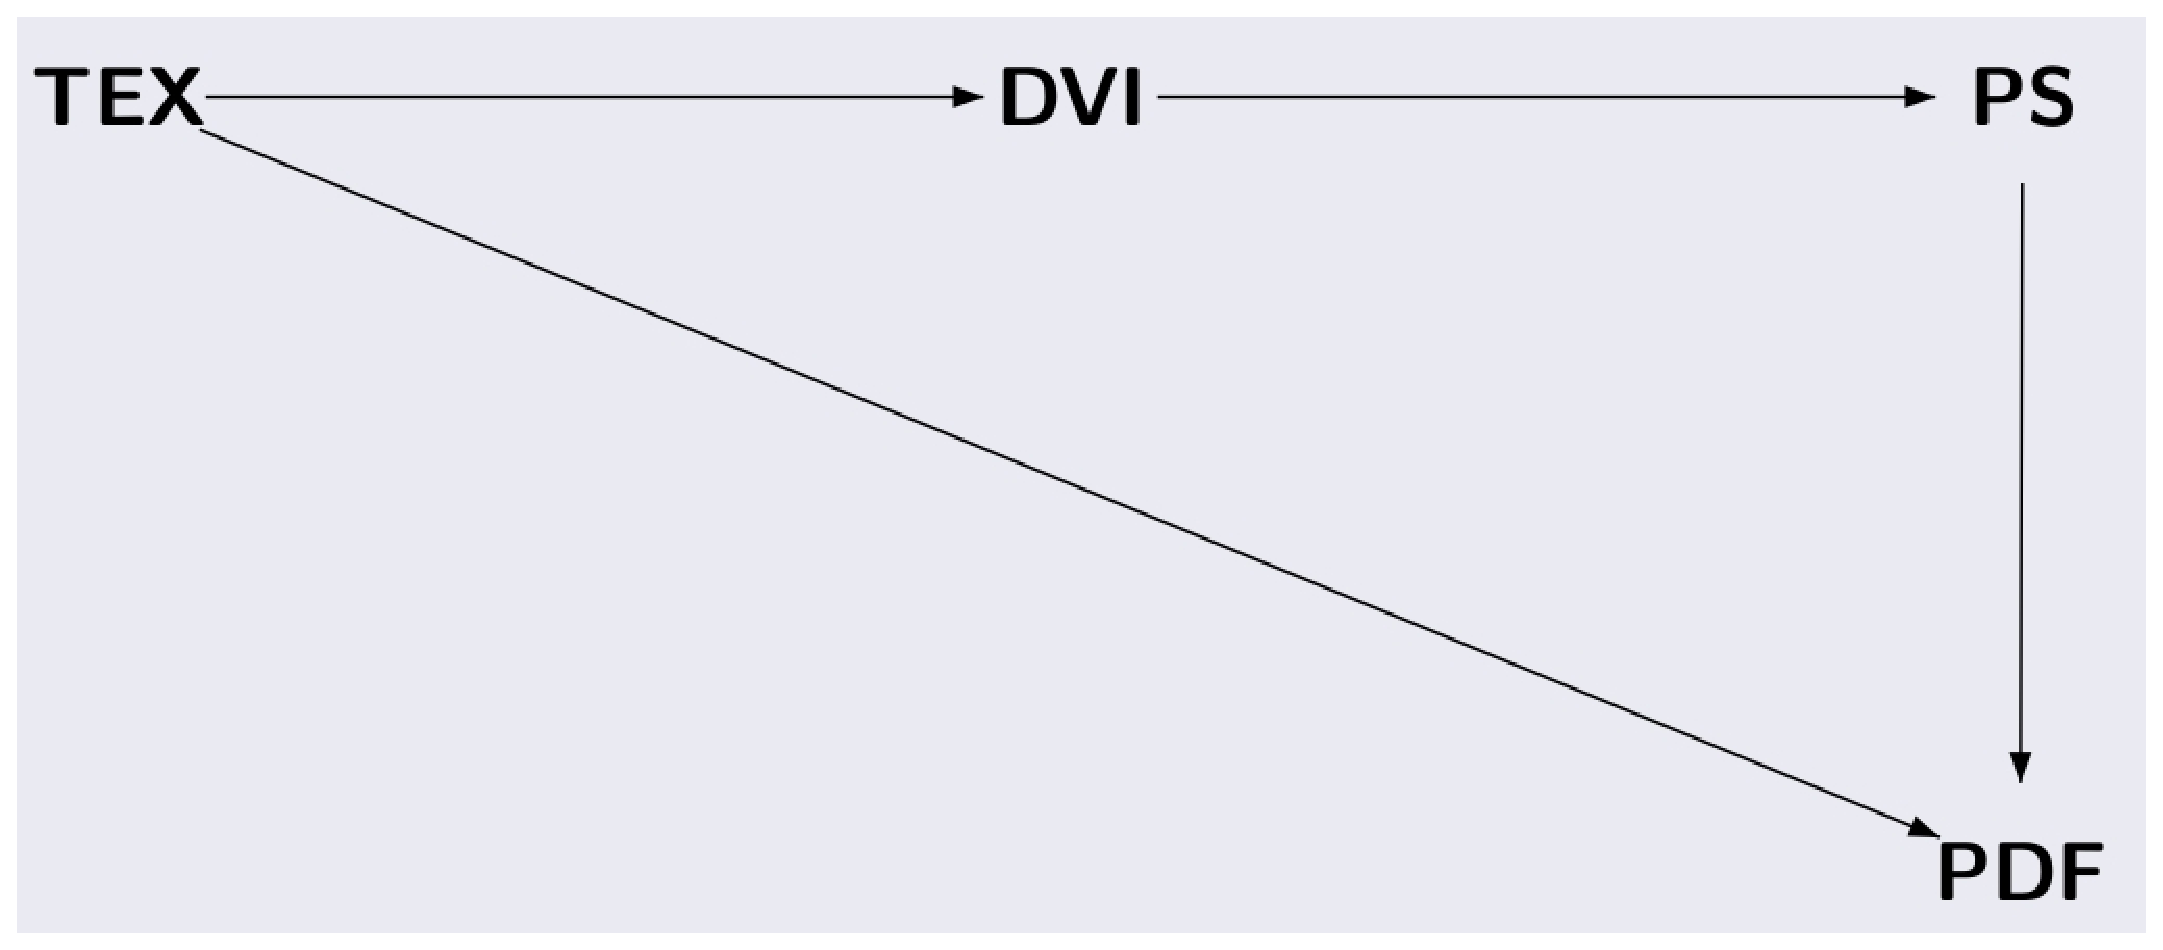
\includegraphics[width=0.8\textwidth]{images/Auswahl_049.eps}
  \end{figure}
	\end{block}
\end{frame}

\begin{frame}[fragile]
	\frametitle{Übersetzung}
	\begin{block}{Quelltext kompilieren}
		\begin{verbatim}
			latex TeXDatei.tex
			pdflatex TeXDatei.tex
		\end{verbatim}
	\end{block}
\end{frame}

\begin{frame}[fragile]
	\frametitle{Übersetzung mit latex}
	\begin{block}{Quelltext kompilieren}
		\begin{verbatim}
			latex TeXDatei.tex

			dvips TeXDatei.dvi

			ps2pdf TeXDatei.ps
		\end{verbatim}
	\end{block}
\end{frame}

\begin{frame}[fragile]
	\frametitle{Übersetzung mit pdflatex}

	Da es für den Anfang komplett ausreichend ist werden wir pdflatex verwenden.
	\pause
	\begin{block}{Quelltext kompilieren}
		\begin{verbatim}
			pdflatex TeXDatei.tex
		\end{verbatim}
	\end{block}
	\pause
	\begin{alertblock}{Achtung}
		Für Fortgeschrittene: Einfach einzubinden kann aber keinen \textit{gastex} Code interpretieren!
	\end{alertblock}
\end{frame}




% Editoren
\subsection{Editoren}

\begin{frame}
	\frametitle{Eine kleine Auswahl}
	\begin{block}{Windows}
		\begin{itemize}
			\item TeXstudio
			\item TEXnicCenter
		\end{itemize}
	\end{block}
	\pause
	\begin{block}{Linux}
		\begin{itemize}
			\item TeXstudio
			\item TEXMaker
			\item Konsole
		\end{itemize}
	\end{block}
	\pause
	\begin{block}{Mac}
		\begin{itemize}
			\item Wie unter Linux
		\end{itemize}
	\end{block}
\end{frame}

\section{Grundlagen}


% Grundgerüst für Dokument
\subsection{Dokumentengrundgerüst}

\begin{frame}[fragile]
	\frametitle{Dokumentengrundgerüst}

	\begin{block}{Grundgerüst}
		\begin{verbatim}
\documentclass{scrbook}
\usepackage{ngerman}[babel]
\usepackage[utf8]{inputenc}
\usepackage[T1]{fontenc}
\usepackage[a4paper]{geometry}
% Weitere Packete

% Definitionen

\begin{document}
	% Inhalt des Dokuments
\end{document}
		\end{verbatim}
	\end{block}
\end{frame}



% Text strukturieren, chapters, sections etc.
\subsection{Text strukturieren}

\begin{frame}[fragile]
	\frametitle{Gliederungen}

  \begin{block}{Code}
    \begin{verbatim}
\section{Abschnitt 1}
  \subsection{Unterabschnitt 1.1}
  \subsection{Unterabschnitt 1.2}
    \subsubsection{Unterabschnitt 1.2.1}
\section{Abschnitt 2}
  \subsection{Unterabschnitt 2.1}
    \end{verbatim}
  \end{block}
\end{frame}

\begin{frame}
  \frametitle{Gliederungen - Resultat}

  \begin{block}{Resultat}
    Probieren wir das doch gleich mal aus ...
  \end{block}
\end{frame}

\begin{frame}[fragile]
	\frametitle{Inhaltsverzeichnis}

  \begin{block}{Vorteile}
  	\begin{itemize}[<+->]
  		\item Automatische Generierung
  		\item Auf Wunsch im Dokument selbst Verlinkung auf die Seiten
  		\item (pdf)latex Befehl muss zwei mal aufgerufen werden
  	\end{itemize}
  \end{block}
  \pause
	\begin{block}{Code}
		\begin{verbatim}
\tableofcontents
    \end{verbatim}
	\end{block}
\end{frame}

\begin{frame}
	\frametitle{Resultat}

  \begin{figure}
    \centering
    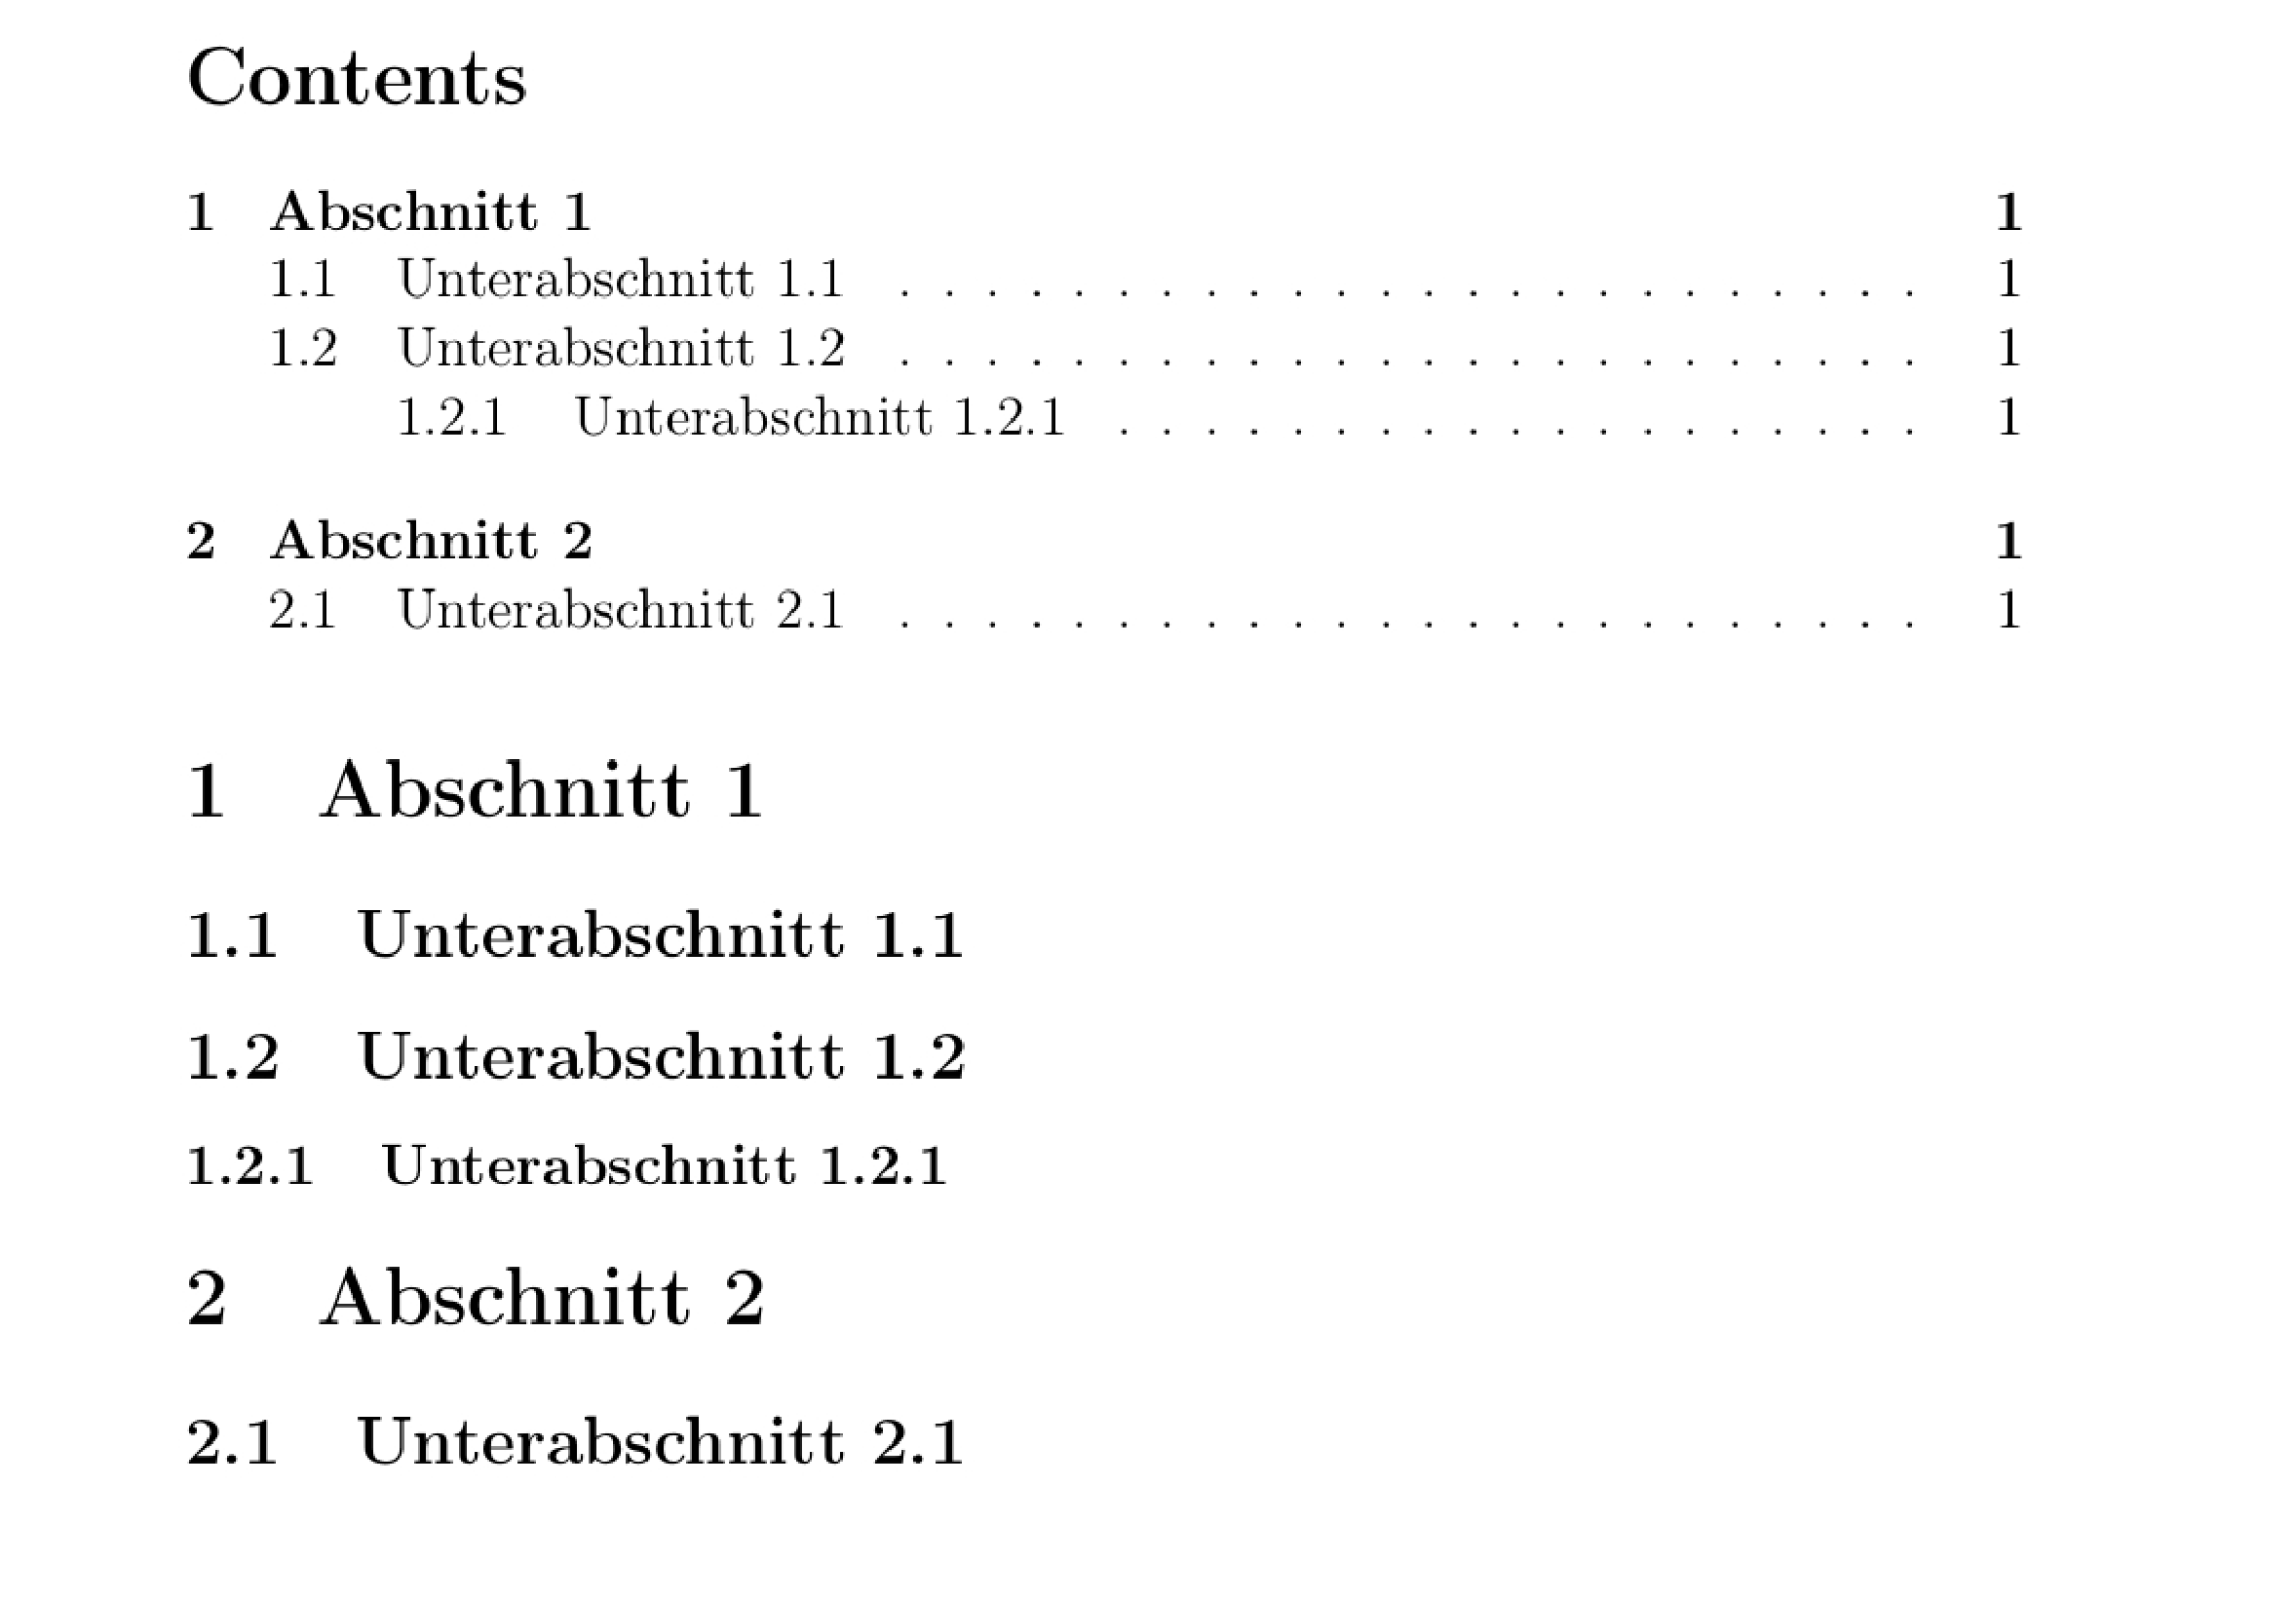
\includegraphics[width=0.8\textwidth]{images/TableOfContents.eps}
  \end{figure}
%  \end{block}
\end{frame}


\subsection{Texte formatieren}

\begin{frame}[fragile]
	\frametitle{Textstile}

	\begin{example}
		\begin{itemize}[<+->]
			\item Ein \textbf{fetter Text}
			\item Ein \textit{kursiver Text}
		\end{itemize}
	\end{example}
  \pause
  \begin{block}{Code}
    \begin{verbatim}
\begin{itemize}
  \item Ein \textbf{fetter Text}
  \item Ein \textit{kursiver Text}
\end{itemize}
    \end{verbatim}
  \end{block}
\end{frame}

\begin{frame}[fragile]
  \frametitle{Textfarbe}

  \begin{example}
    \textcolor{red}{rot}

    \textcolor[rgb]{0.8,0.1,0.8}{lila}
  \end{example}
  \pause
  \begin{block}{Code}
    \begin{verbatim}
\textcolor{red}{rot}

\textcolor[rgb]{0.8,0.1,0.8}{lila}
    \end{verbatim}
  \end{block}
\end{frame}



\begin{frame}[fragile]
  \frametitle{Schriftart ändern}

  \begin{example}
    \textsc{Kapit\"alchen}
    \textsf{Sans Serif}
    \textrm{Roman}
    \texttt{Schreibmaschine}
    \textnormal{Normale Schrift} 
  \end{example}
  \pause
  \begin{block}{Code}
    \begin{verbatim}
\textsc{Kapit\"alchen}
\textsf{Sans Serif}
\textrm{Roman}
\texttt{Schreibmaschine}
\textnormal{Normale Schrift} 
    \end{verbatim}
  \end{block}
\end{frame}
\begin{frame}[fragile]
  \frametitle{Schriftart ändern}

  Wenn man nun aber dauerthaft serifenlos schreiben möchte?

  \pause
  \begin{block}{Code}
    \begin{verbatim}
\renewcommand{\familydefault}{\sfdefault}
    \end{verbatim}
  \end{block}
\end{frame}

\begin{frame}[fragile]
  \frametitle{Anführungszeichen}

  \pause
  \begin{block}{Zitat Dr. Evil}
    Back in the 60's, I had a weather changing machine that was, in essence, a sophisticated heat beam which we called a \glqq laser\grqq. Using these \glq lasers\grq, we punch a hole in the protective layer around the Earth, which we scientists call the \flqq Ozone Layer\frqq.
  \end{block}
  \pause
  \begin{block}{Code}
    \begin{verbatim}
      Back in the 60's, [...] called a \glqq laser\grqq. 
      Using these \glq lasers\grq, we punch [...] call 
      the \flqq Ozone Layer\frqq.
    \end{verbatim}
  \end{block}
\end{frame}

\begin{frame}
  \frametitle{Ausrichtung}

  \begin{example}
    \begin{center}
      Zentrierter Text
    \end{center}
    \pause
    \begin{flushleft}
      Zentrierter Text
    \end{flushleft}
    \pause
    \begin{flushright}
      Zentrierter Text
    \end{flushright}
  \end{example}
\end{frame}
\begin{frame}[fragile]
	\frametitle{Ausrichtung}

	\begin{block}{Code}
		\begin{verbatim}
\begin{center}
	Zentrierter Text
\end{center}
\begin{flushleft}
	Zentrierter Text
\end{flushleft}
\begin{flushright}
	Zentrierter Text
\end{flushright}
		\end{verbatim}
	\end{block}
\end{frame}

\begin{frame}[fragile]
	\frametitle{Textgröße}

  \begin{example}
    \Huge{Huge}
    \huge{huge}
    \small{small}
  \end{example}

	\begin{block}{Größen}
		\begin{verbatim}
\Huge{Huge}
\huge{huge}
\small{small}
		\end{verbatim}
	\end{block}
\end{frame}


% AUFZÄHLUNGEN
\begin{frame}[fragile]
	\frametitle{Aufzählungen}

  \begin{example}
    \begin{itemize}
      \item Item 1
      \item Item 2
      \item Item 3
    \end{itemize}
  \end{example}

  \pause

  \begin{block}{Code}
    \begin{verbatim}
\begin{itemize}
  \item Item 1
  \item Item 2
  \item Item 3
\end{itemize}
    \end{verbatim}
  \end{block}
\end{frame}
\begin{frame}[fragile]
  \frametitle{Aufzählungen 2}

  \begin{example}
    \begin{itemize}
      \item[\checkmark] Item 1
      \item[\checkmark] Item 2
      \item[\checkmark] Item 3
    \end{itemize}
  \end{example}

  \pause

  \begin{block}{Code}
    \begin{verbatim}
\begin{itemize}
  \item[\checkmark] Item 1
  \item[\checkmark] Item 2
  \item[\checkmark] Item 3
\end{itemize}
    \end{verbatim}
  \end{block}
\end{frame}

\begin{frame}[fragile]
  \frametitle{Aufzählungen}

  \begin{example}
    \begin{enumerate}
      \item Item 1
      \item Item 2
      \item Item 3
    \end{enumerate}
  \end{example}

  \begin{block}{Code}
    \begin{verbatim}
\begin{enumerate}
  \item Item 1
  \item Item 2
  \item Item 3
\end{enumerate}
    \end{verbatim}
  \end{block}
\end{frame}
\begin{frame}[fragile]
  \frametitle{Aufzählungen}

  \begin{example}
    \begin{itemize}
      \item Item 1
        \begin{itemize}
          \item Sub-Item 1
          \item Sub-Item 2
        \end{itemize}
      \item Item 2
      \item Item 3
    \end{itemize}
  \end{example}
  \pause
  \begin{block}{Code}
    \begin{verbatim}
\begin{itemize}
  \item Item 1
    \begin{itemize}
      \item Sub-Item 1
      \item Sub-Item 2
    \end{itemize}
  \item Item 2
  \item Item 3
\end{itemize}
    \end{verbatim}
  \end{block}
\end{frame}






% ABSTÄNDE

\begin{frame}[fragile]
	\frametitle{Abstände}

	\begin{block}{Abstände}
    \begin{itemize}[<+->]
      \item Explizite Leerzeichen: \lstinline{~}
      \item Explizite Zeilenumbrüche: \lstinline{\\}
      \item Expliziter Seitenumbruch: \lstinline{\newpage}
      \item Horizontal, vertikal Auffüllen: \lstinline{\hfill} oder \lstinline{\vfill}
    \end{itemize}
	\end{block}
\end{frame}


% Tabellen einfügen
\subsection{Tabellen}

\begin{frame}[fragile]
  \frametitle{Tabellen}

  \begin{example}
    \begin{tabular}{cc}
      Ich & bin \\
      eine & Tabelle
    \end{tabular}
  \end{example}
  \pause
  \begin{block}{Code}
    \begin{verbatim}
\begin{tabular}{cc}
  Ich & bin \\
  eine & Tabelle
\end{tabular}
    \end{verbatim}
  \end{block}
\end{frame}
\begin{frame}[fragile]
  \frametitle{Tabellen - Orientierungen}

  \begin{example}
    \begin{tabular}{rl}
      Ich & bin \\
      eine & Tabelle
    \end{tabular}
  \end{example}
  \pause
  \begin{block}{Code}
    \begin{verbatim}
\begin{tabular}{rl}
  Ich & bin \\
  eine & Tabelle
\end{tabular}
    \end{verbatim}
  \end{block}
\end{frame}
\begin{frame}[fragile]
  \frametitle{Tabellen - Rahmen}

  \begin{example}
    \begin{tabular}{|c|c|}
      Ich & bin \\
      \hline
      eine & Tabelle \\
      \hline
    \end{tabular}
  \end{example}
  \pause
  \begin{block}{Code}
    \begin{verbatim}
\begin{tabular}{|c|c|}
  Ich & bin \\
  \hline
  eine & Tabelle \\
  \hline
\end{tabular}
    \end{verbatim}
  \end{block}
\end{frame}
\begin{frame}[fragile]
  \frametitle{Tabellen - Caption}

  \begin{example}
    \begin{table}
      \begin{tabular}{|c|c|}
        Ich & bin \\
        \hline
        eine & Tabelle \\
        \hline
      \end{tabular}
      \caption{Dies ist eine einfache Tabelle}
    \end{table}
  \end{example}
  \pause
  \begin{block}{Code}
    \begin{verbatim}
\begin{table}
  \begin{tabular}{|c|c|}
    Ich & bin \\
    \hline
    eine & Tabelle \\
    \hline
  \end{tabular}
  \caption{Dies ist eine einfache Tabelle}
\end{table}
    \end{verbatim}
  \end{block}
\end{frame}
\begin{frame}[fragile]
  \frametitle{Tabellen - Referenz}

  \begin{example}
    \begin{table}
      \begin{tabular}{|c|c|}
        Ich & bin \\
        \hline
        eine & Tabelle \\
        \hline
      \end{tabular}
      \label{myTable1}
    \end{table}
  \end{example}
  \pause

  \begin{block}{Code}
    \begin{verbatim}
\begin{table}
  \begin{tabular}{|c|c|}
    Ich & bin \\
    \hline
    eine & Tabelle \\
    \hline
  \end{tabular}
  \label{myTable1}
\end{table}
    \end{verbatim}
  \end{block}
\end{frame}

\begin{frame}[fragile]
  \begin{block}{Verwendung}
    Nun können wir einfach unsere Tabelle \ref{myTable1} referenzieren.
  \end{block}
  \pause
  \begin{block}{Code}
    \begin{verbatim}
Nun können wir einfach unsere Tabelle \ref{myTable1}
referenzieren.
    \end{verbatim}
  \end{block}
\end{frame}

\subsection{Mathematische Formeln}

\begin{frame}[fragile]
  \frametitle{Zusätzliche Pakete}

  Bevor wir mathematische Symbole verwenden können müssen wir erst noch die entsprechenden Pakete hinzufügen.

  \begin{block}{Code}
    \begin{verbatim}
\usepackage{amssymb}
\usepackage{amsmath} 
\usepackage{amsfonts}
    \end{verbatim}
  \end{block}
\end{frame}

\begin{frame}[fragile]

  \begin{block}{Formeln kennzeichnen}
    Formeln müssen im Text extra gekennzeichnet werden, ansonsten kann es auch sein dass das Dokument nicht kompiliert.
  \end{block}
  \pause
  \begin{block}{Code}
    \begin{verbatim}
$ Hier die Formel $
    \end{verbatim}

  \end{block}
\end{frame}

\begin{frame}[fragile]
  \frametitle{Formeln platzieren}
	\begin{example}
		Im Text: $ Y_l^m(\vartheta, \varphi) = N_l^m\cdot P_l^m(cos\vartheta)\cdot e^{im\varphi} $
  \end{example}
  \pause
  \begin{block}{Code}
		\begin{verbatim}
Im Text: $ Y_l^m(\vartheta, \varphi) = N_l^m\cdot
P_l^m(cos\vartheta)\cdot e^{im\varphi} $
		\end{verbatim}

	\end{block}
\end{frame}

\begin{frame}[fragile]
  \frametitle{Formeln platzieren}
  \begin{example}
    Nicht im Text: $$ Y_l^m(\vartheta, \varphi) = N_l^m\cdot P_l^m(cos\vartheta)\cdot e^{im\varphi} $$
  \end{example}
  \pause
  \begin{block}{Code}
	 \begin{verbatim}
Nicht im Text: $$ Y_l^m(\vartheta, \varphi) = N_l^m\cdot
P_l^m(cos\vartheta)\cdot e^{im\varphi} $$
		\end{verbatim}
	\end{block}
\end{frame}

\begin{frame}[fragile]
  \frametitle{Griechische Buchstaben}
  \begin{example}
    Ein phi bitte: $ \phi $ \\
    Nein, ein großes phi bitte: $ \Phi $
  \end{example}
  \pause
  \begin{block}{Code}
   \begin{verbatim}
Ein phi bitte: $ \phi $ \\
Nein, ein großes phi bitte: $ \Phi $
    \end{verbatim}
  \end{block}
\end{frame}

\begin{frame}[fragile]
  Ein Beweisende kenntlich machen.
  \begin{example}
    Beweis hier einfügen.
    \hfill $\square$
  \end{example}
  \pause
  \begin{block}{Code}
    \begin{verbatim}
Beweis hier einfügen.
\hfill $\square$
    \end{verbatim}
  \end{block}
\end{frame}

\subsection{Bilder, Grafiken, Referenzen}

\begin{frame}[fragile]
  \frametitle{Das graphicx Paket}

  \LaTeX kann Bilder nicht sofort verwenden und verstehen, hierfür ist ein weiteres Paket nötig.
  \pause
  \begin{block}{LaTeX Code}
    \begin{verbatim}
      \usepackage{graphicx}
    \end{verbatim}
  \end{block}
  \pause
  \begin{block}{Kompilieren mit Bildern}
    \begin{itemize}
      \item Wenn mit \textit{latex} kompiliert wird können nur \textbf{EPS} Dateien verwendet werden.
      \item Wenn mit \textit{pdflatex} kompiliert wird können alle gängigen Bildformate verwendet werden.
    \end{itemize}
  \end{block}
\end{frame}

\begin{frame}[fragile]
  \frametitle{Bilder einbinden}

  \begin{example}
    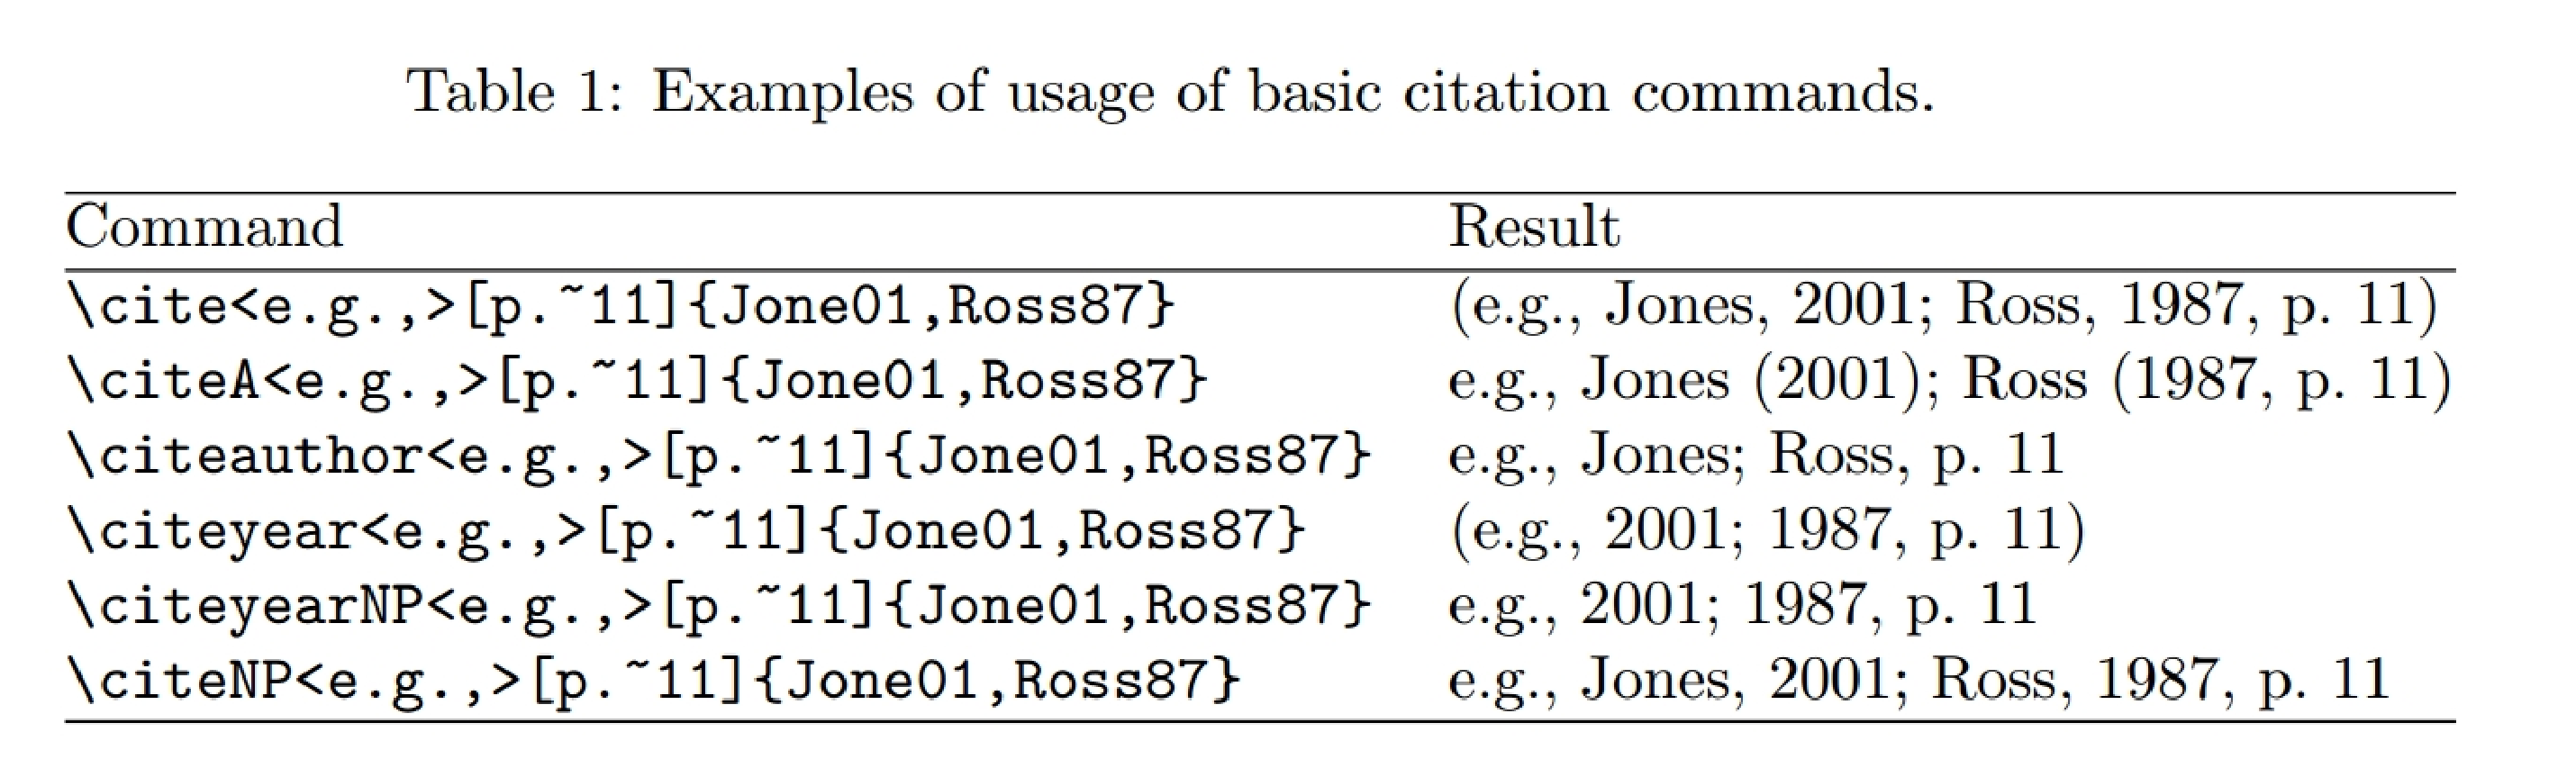
\includegraphics[width = 0.9\textwidth]{images/Auswahl_047.eps}
  \end{example}
	\pause
	\begin{block}{LaTeX Code}
		\begin{verbatim}
			\includegraphics[width = 0.9\textwidth]{images/example.eps}
		\end{verbatim}
	\end{block}
\end{frame}
\begin{frame}[fragile]
  \frametitle{Bilder einbinden - 2}

	\begin{block}{Optionen}
		Wir haben as \textit{width} Commando in den [ ] Klammern gesehen. Es gibt hier noch ein paar mehr, die jedoch alle optional sind.

		\begin{tabular}{|l|l|}
			\textbf{Commando} & \textbf{Erklärung} \\
			\hline\hline
			width=xx & Breite des Bildes (führt eine Skalierung durch) \\\hline
			height=xx & Höhe des Bildes (führt eine Skalierung durch) \\\hline
			scale=xx & Gleichmässige Skalierung für x und y \\\hline
			angle=xx & Dreht das Bild counter-clockwise um xx Grad \\\hline
		\end{tabular}
	\end{block}
\end{frame}

\begin{frame}[fragile]
	\frametitle{Bilder - Caption und Label}

  \begin{block}{Caption und Label}
	\begin{itemize}[<+->]
		\item Bereits aus den Tabellen bekannt: \textit{caption} und \textit{label}
		\item Können beide auch für Bilder verwendet werden, ...
		\item ... was jedoch eine leichte Anpassung für die Einbindung von Bildern braucht
	\end{itemize}
  \end{block}
\end{frame}

\begin{frame}[fragile]
  \frametitle{Bilder einbinden 2}

  \begin{example}
		\begin{figure}
    	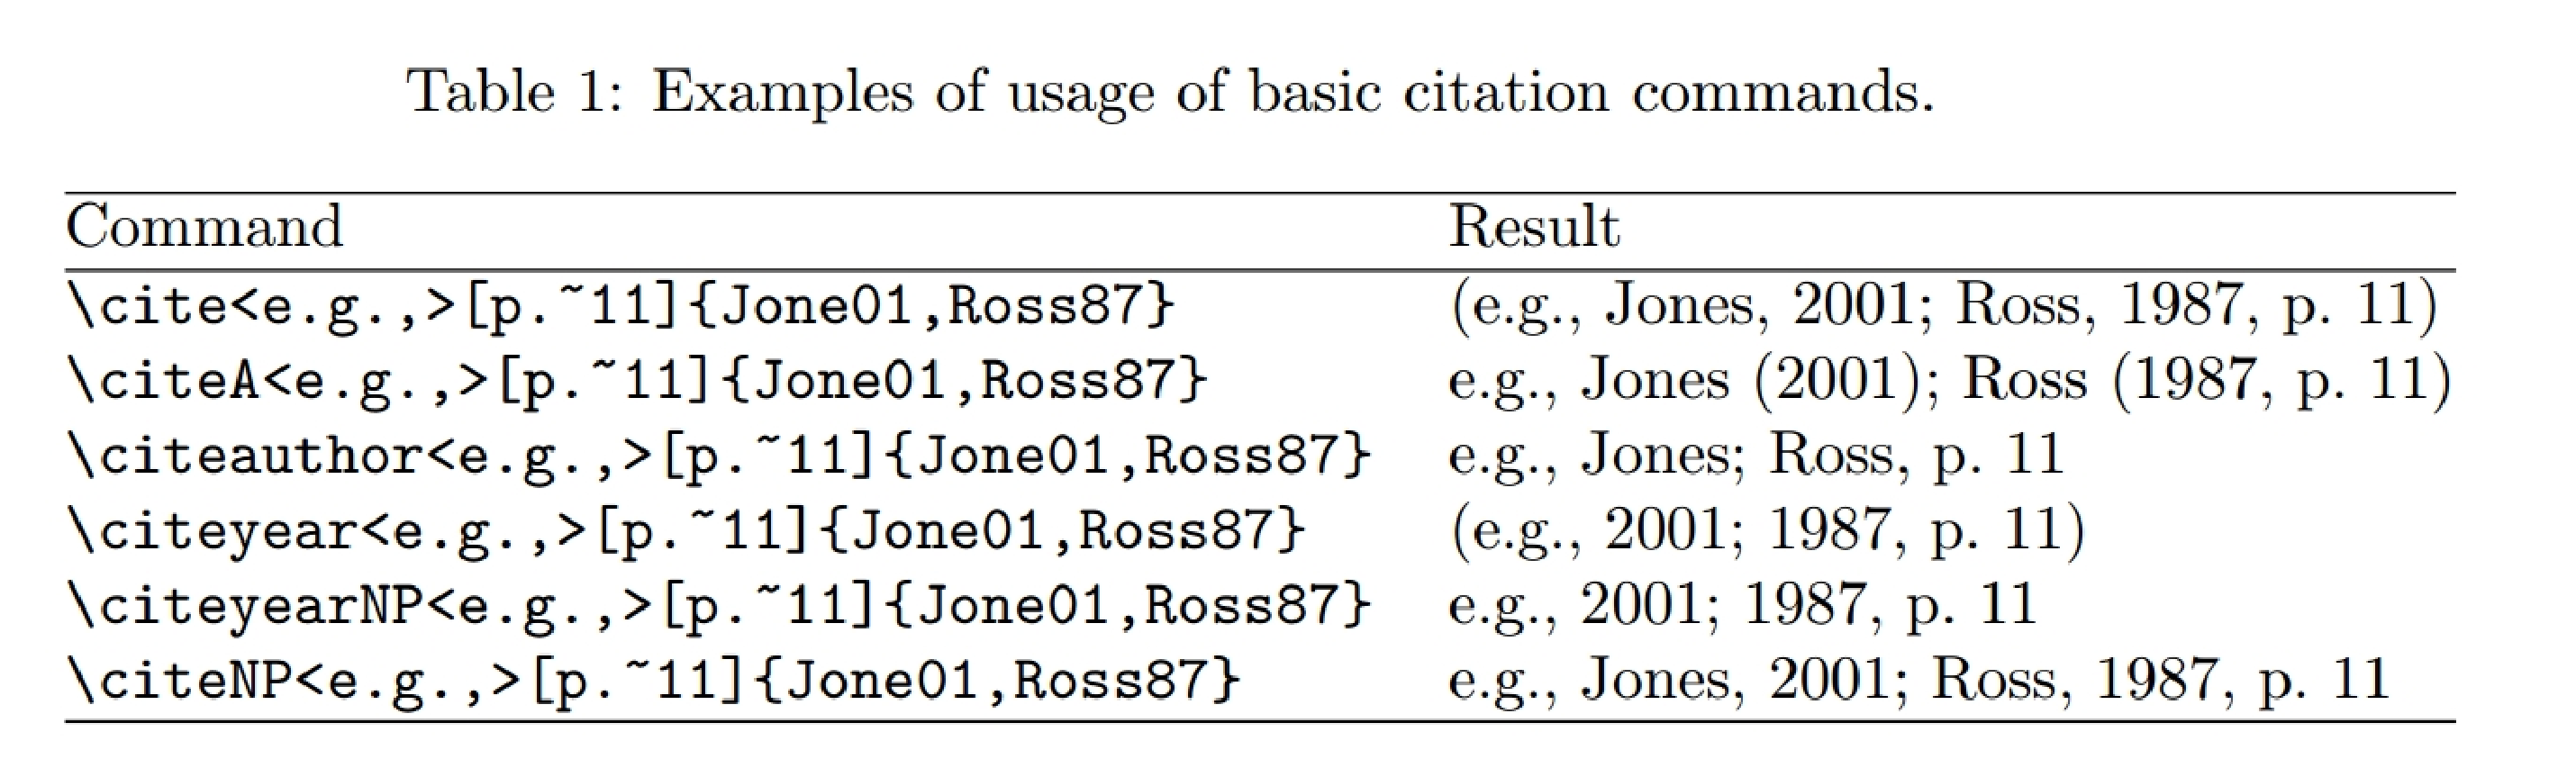
\includegraphics[width = 0.8\textwidth]{images/Auswahl_047.eps}
			\caption{Hier gibt es nichts zu sehen!}
			\label{fig:myFig1}
		\end{figure}
  \end{example}
	\pause
	\begin{block}{LaTeX Code}
		\begin{verbatim}
\begin{figure}
	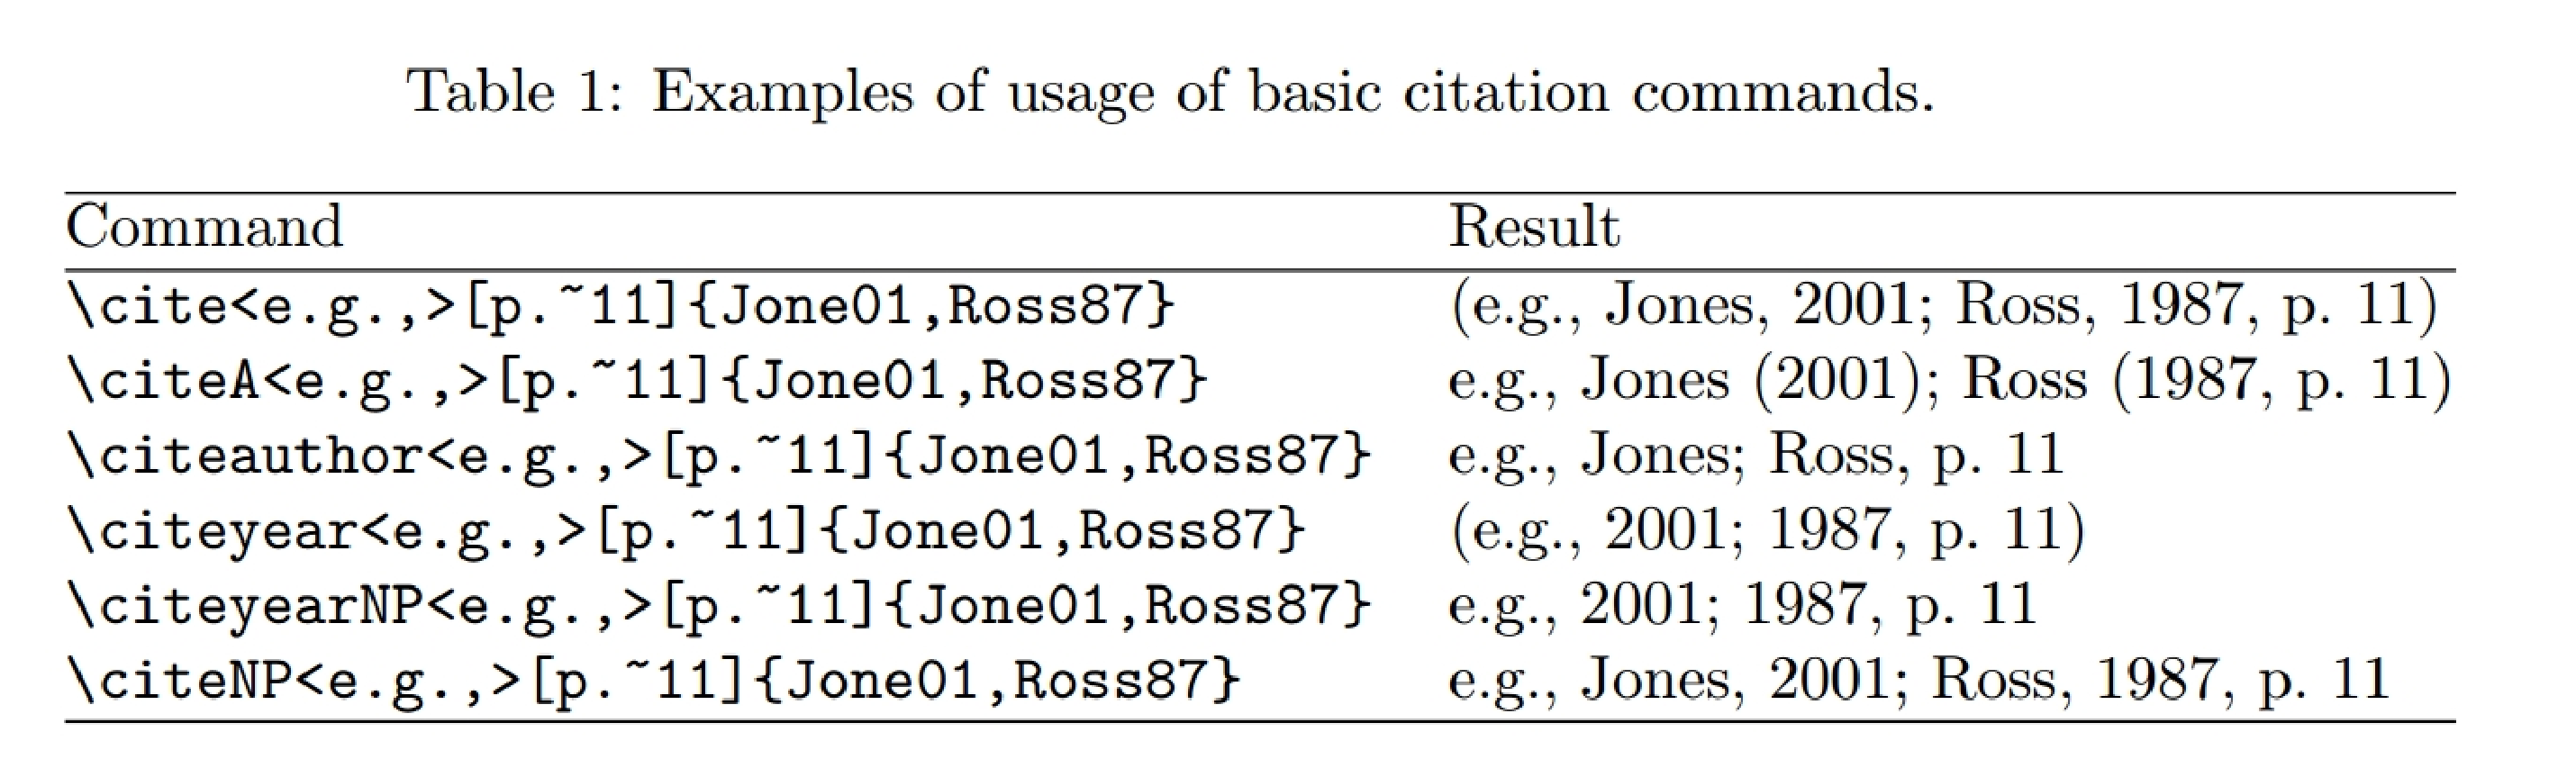
\includegraphics[width = 0.8\textwidth]{images/Auswahl_047.eps}
	\caption{Hier gibt es nichts zu sehen!}
	\label{fig:myFig1}
\end{figure}
		\end{verbatim}
	\end{block}
\end{frame}

\begin{frame}[fragile]
	\frametitle{Bilder referenzieren}

	Bilder können nun wie von Tabellen bekannt im Text referenziert werden.
	\pause
	\begin{example}
		Wie man in Abbildung \ref{fig:myFig1} sehen kann sieht man nichts.
	\end{example}
	\pause
	\begin{block}{LaTeX Code}
		\begin{verbatim}
Wie man in Abbildung \ref{fig:myFig1} sehen kann sieht man nichts.
		\end{verbatim}
	\end{block}
\end{frame}







\subsection{Diagramme}
% DIAGRAMME
\begin{frame}
  \frametitle{Diagramme}

  \begin{block}{Wie bindet man Diagramme}
    \begin{itemize}[<+->]
      \item Möglichkeit 1: Diagramme von anderen Programmen, wie SPSS ploten lassen und einfach nur noch einbinden
      \item Möglichkeit 2: Diagramme über \textit{tikz} generieren und von \LaTeX ploten lassen
      \item<1> {\color{red}Einfach und schnell, sieht jedoch manchmal etwas verpixelt aus.}
      \item<2> {\color{red}Etwas aufwendiger, verbraucht etwas Nerven, dafür aber immer scharfe Bilder}
    \end{itemize}
  \end{block}
\end{frame}
\begin{frame}
  \frametitle{Diagramme}

  \begin{example}
    \begin{tikzpicture}
      \begin{axis}[title  = Beispiel Balkendiagram,
        xbar,
        y axis line style = { opacity = 0 },
        axis x line       = none,
        tickwidth         = 0pt,
        enlarge y limits  = 0.2,
        enlarge x limits  = 0.02,
        symbolic y coords = {LaTeX, Tools, Distributions, Editors},
        nodes near coords,
      ]
      \addplot coordinates { (57727,LaTeX)         (5672,Tools)
                             (2193,Distributions)  (11106,Editors) };
      \addplot coordinates { (14320,LaTeX)         (1615,Tools)
                             (560,Distributions)   (3075,Editors)  };
      \legend{Topics, Posts}
      \end{axis}
    \end{tikzpicture}
  \end{example}
\end{frame}
\begin{frame}[fragile]
  \frametitle{Diagramme}

  \begin{block}{Code}
    \begin{verbatim}
\begin{tikzpicture}
  \begin{axis}[title  = Beispiel Balkendiagram,
    xbar,
    y axis line style = { opacity = 0 },
    axis x line       = none,
    tickwidth         = 0pt,
    enlarge y limits  = 0.2,
    enlarge x limits  = 0.02,
    symbolic y coords = {LaTeX, Tools, Distributions, Editors},
    nodes near coords,
  ]
  \addplot coordinates { (57727,LaTeX)         (5672,Tools)
                         (2193,Distributions)  (11106,Editors) };
  \addplot coordinates { (14320,LaTeX)         (1615,Tools)
                         (560,Distributions)   (3075,Editors)  };
  \legend{Topics, Posts}
  \end{axis}
\end{tikzpicture}
    \end{verbatim}
  \end{block}
\end{frame}

\begin{frame}[fragile]
  \frametitle{Tikz}

  \begin{block}{Tikz}
    \begin{itemize}[<+->]
      \item \textit{Tikz} ist hinreichend kompliziert, aber es gibt genug Beispiele an denen man lernen kann.
      \item Webseite: \url{http://www.texample.net/tikz/examples/}
      \item Und es gibt genug Tools die Tikz Code generieren können:
      \item Webseite: \url{http://www.texample.net/tikz/resources}
      \item Trotzdem für den Anfang sehr schwer handhabbar
    \end{itemize}
  \end{block}
\end{frame}


% Referenzen, Verweise
\subsection{Verweise}

\begin{frame}[fragile]
	\frametitle{Variante 1: Der einfache Weg}

  \begin{example}
  Siehe \cite{ R05} und \cite{ M05}. %Zitat


      \begin{thebibliography}{n} %Verzeichnis
        \bibitem[Rie05]{R05} S.Rieger: \emph{Einführung in
LaTeX},Vortrag am I2
        \bibitem[Mai05]{M05} H.Maier: \emph{Seminararbeit}
\end{thebibliography}
  \end{example}
  \pause
	\begin{block}{Literaturverzeichnis 1}
		\begin{verbatim}
			Siehe \cite{ R05} und \cite{ M05}. %Zitat


			\begin{thebibliography}{n} %Verzeichnis
 				\bibitem[Rie05]{R05} S.Rieger: \emph{Einführung in
LaTeX},Vortrag am I2
 				\bibitem[Mai05]{M05} H.Maier: \emph{Seminararbeit}
\end{thebibliography}
		\end{verbatim}
	\end{block}
\end{frame}



\begin{frame}[fragile]
  \frametitle{Variante 2: Etwas schwieriger}

  \begin{block}{Literaturverzeichnis 1}
    \begin{verbatim}
      Siehe \cite{ R05} und \cite{ M05}. %Zitat


      \begin{thebibliography}{n} %Verzeichnis
        \bibitem[Rie05]{R05} S.Rieger: \emph{Einführung in
LaTeX},Vortrag am I2
        \bibitem[Mai05]{M05} H.Maier: \emph{Seminararbeit}
\end{thebibliography}
    \end{verbatim}
  \end{block}
\end{frame}

\begin{frame}[fragile]
  \frametitle{Nach APA zitieren}

  \begin{block}{Zusätzliches Package}
    \begin{verbatim}
      \usepackage[options]{apacite}
    \end{verbatim}
  \end{block}
  \pause
  \begin{block}{apacite}
    Liste von Optionen kann unter \url{ftp://ftp.dante.de/pub/tex/biblio/bibtex/contrib/apacite/apacite.pdf} gefunden werden.
  
  \end{block}
\end{frame}
\begin{frame}[fragile]
  \frametitle{Nach APA zitieren - 2}

  \begin{block}{Zusätzliches Package}
    \begin{verbatim}
      \bibliographystyle{apacite}
      \bibliography{bibfiles}
    \end{verbatim}
  \end{block}
  \pause
  \begin{block}{bibliographystyle}
    Beschreibt den Stil der verwendet werden soll.
    \begin{tabular}{c|c|c|c}
      apacite & apacitex & apacann & apacannx
    \end{tabular}
  \end{block}
  \pause
  \begin{block}{bibliography}
    Liste aller *.bib Dateien die BibTeX Code enthält (hierzu gleich mehr).
  \end{block}
\end{frame}

\begin{frame}[fragile]
  \frametitle{Was ist BibTex Code?}
  \pause
  \begin{example}
    \url{https://scholar.google.de/scholar?hl=de&q=Latex+cookbook&btnG=&lr=}
  \end{example}
  \pause
  \begin{block}{BibTex}
    \begin{verbatim}
@article{lawden1997latex,
  title={LaTeX Cookbook},
  author={Lawden, MD and Charles, Anne},
  journal={Starlink Cookbook 9},
  volume={9},
  year={1997}
}
    \end{verbatim}
  \end{block}
\end{frame}

\begin{frame}[fragile]
  \frametitle{Und nun?}
  \pause
  Wir hatten
  \begin{block}{BibTex}
    \begin{Verbatim}[commandchars=\\\{\}]
@article {\color{red}lawden1997latex}
    \end{Verbatim}
  \end{block}
  \pause
  \begin{example}
    Wir haben bereits \textit{cite} gesehen.

    \textit{apacite} hat hier ein paar mehr Möglichkeiten:

    \begin{figure}
      \centering
      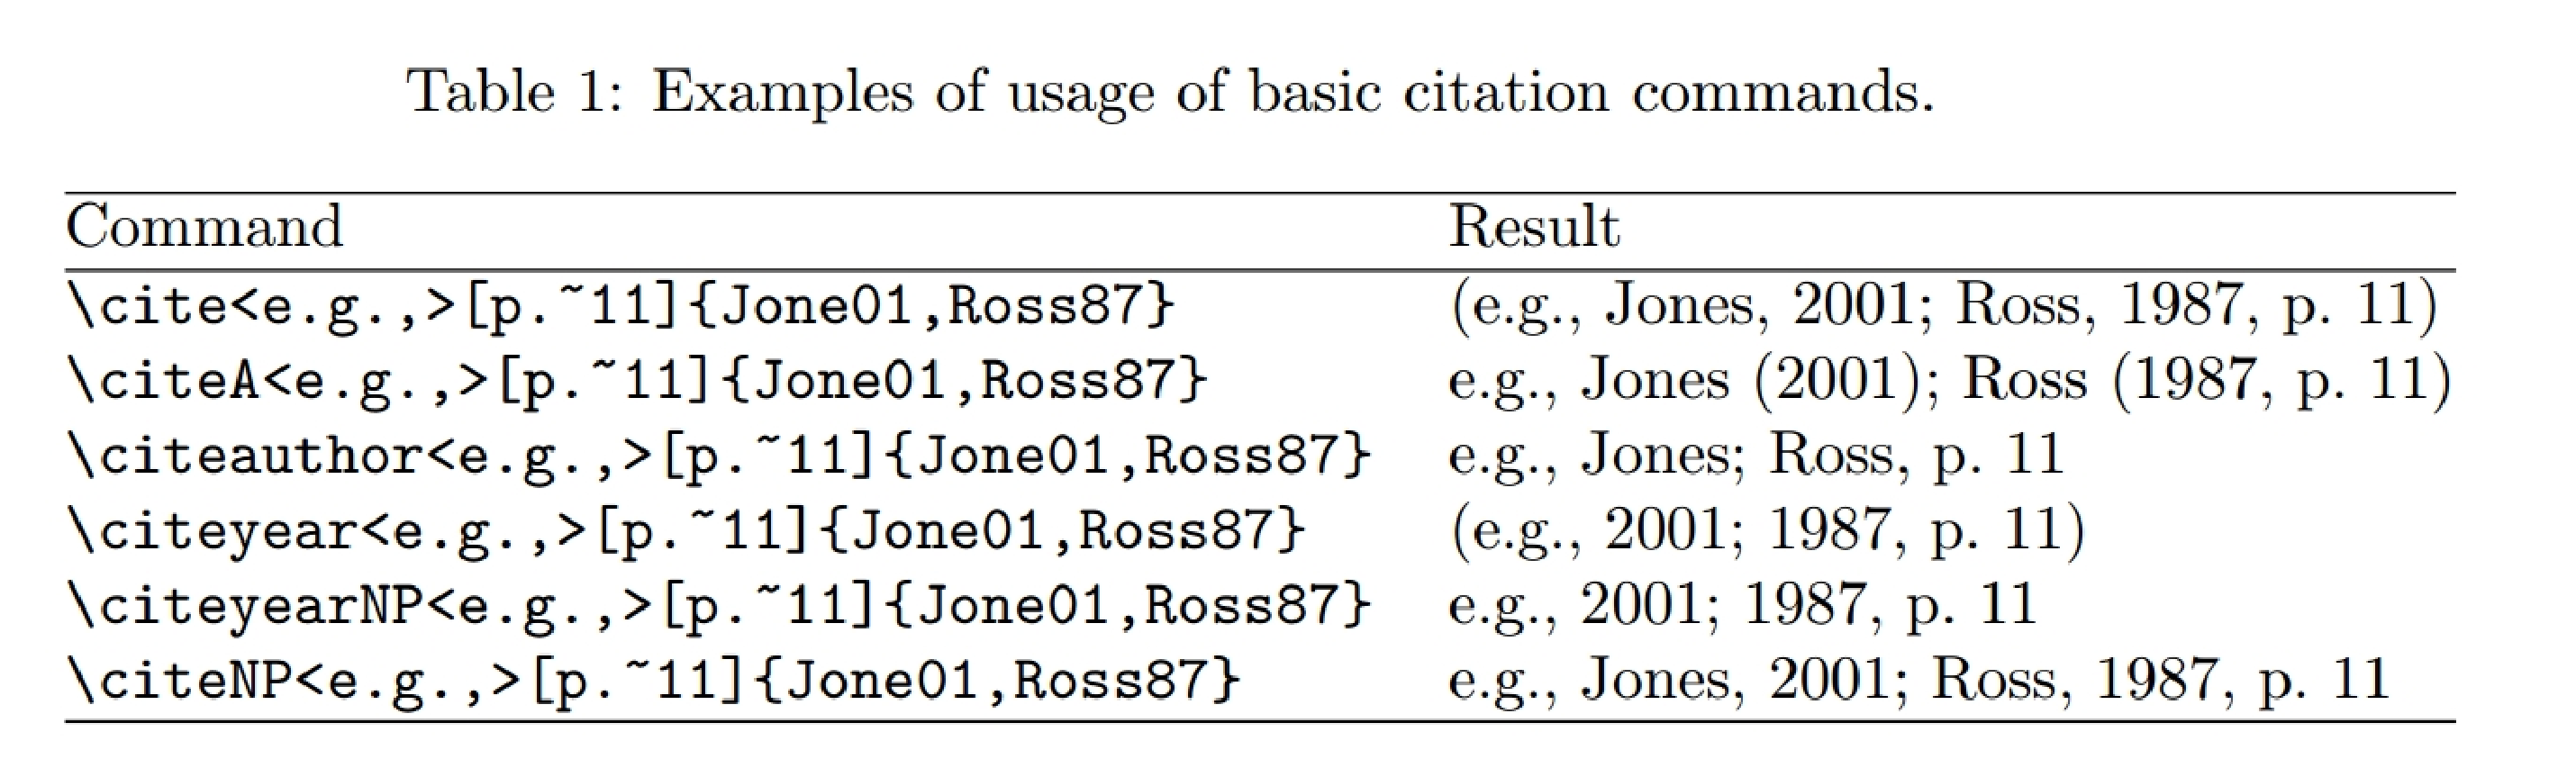
\includegraphics[width = 0.9\textwidth]{images/Auswahl_047.eps}
      \caption{Zitierweisen unter \textit{apacite}}
    \end{figure}

  \end{example}
\end{frame}

% Titelseite
\subsection{Titelseite}

\begin{frame}[fragile]
  \frametitle{Variant 1: Der einfache Weg}

  \begin{block}{Titelseite 1}
    \begin{verbatim}
      \title{Seminarausarbeitung}
      \author {HerbertMaier}
      \date{ \today}
      \maketitle
    \end{verbatim}
  \end{block}
\end{frame}
\begin{frame}
  \frametitle{Variant 1: Der einfache Weg}

  \begin{block}{Resultat - Titelseite 1}
  \end{block}
\end{frame}

\begin{frame}[fragile]
  \frametitle{Variant 2: Eigene Titelseite erstellen}

  \begin{block}{Titelseite 1}
    \begin{verbatim}
\begin{titlepage} \begin{small}
    \vfill {Universität Meine Stadt\\ 
    Institut für \LaTeX \\ 
    Wintersemester 2015/16}
  \end{small}
  \begin{center}
    \begin{Large}
      \vfill {\textsf{\textbf{Meine Hausarbeit}}}
    \end{Large}
  \end{center}
    \begin{small}
    \vfill Dein Name \\ Deine Adresse \\  PLZ Wohnort \\  Email\\ 
    \today
  \end{small}
\end{titlepage}
    \end{verbatim}
  \end{block}
\end{frame}
\section{Beamer}



\subsection{Beamer Klasse}

\begin{frame}[<+->]
  \frametitle{Einleitung}

  \begin{block}{Vorteile}
  \begin{itemize}
    \item Komplexe Formeln stellen keinerlei Probleme dar
    \item Verlinkte Navigationsstrukturen
    \item Mehrere Versionen (Handout, Artikel, etc.)
    \item Erzeugung von PDF Dateien (Gut für Plattformunabgängigkeit)
  \end{itemize}
  \end{block}
\end{frame}


% Themes
\subsection{Themes}

\begin{frame}
  \frametitle{Themes}

  \begin{block}{usetheme}
    Um ein spezielles Theme auszuwählen braucht meein im Kopf der Datei eine weitere Anweisung \lstinline{usetheme{NAME}}.
  \end{block}

  \begin{block}{Standard Themen}
  \centering
	\begin{tabular}{c|c|c|c}
		Antibes & Bergen & Berkeley & Berlin \\\hline
		\textbf{Boadilla} & Copenhagen & Darmstadt & Dresden \\\hline
		Frankfurt & Goettingen & Hannover & Ilmenau \\\hline
		Juanlespins & Madrid & Malmoe & Marburg \\\hline
		Montpellier & Paloalto & Pittsburgh & Rochester \\\hline
		Singapore & Warsaw & &
	\end{tabular}
  \end{block}
\end{frame}

\begin{frame}
  \frametitle{Farbenschemas}

  \begin{block}{usecolortheme}
    Um ein spezielles Farbschema auszuwählen braucht meein im Kopf der Datei eine weitere Anweisung \lstinline{usecolortheme{NAME}}.
  \end{block}

  \begin{block}{Teils verschiedene Farbschemas}
  \centering
  \begin{tabular}{c|c|c|c}
  albatross & beaver & beetle & crane \\\hline
  \textbf{default} & dolphin & dove & fly \\\hline
  lily & orchid & rose & seagull \\\hline
  seahorse & sidebartab & structure & whale \\\hline
  wolverine & &
  \end{tabular}
  \end{block}
\end{frame}


% Folien erzeugen
\subsection{Folien erzeugen}

\begin{frame}[fragile]
  \frametitle{Grundgerüst}
  \begin{block}{Neue \textit{documentclass}}
    \begin{itemize}[<+->]
      \item Wir brauchen eine andere \textit{documentclass}.
      \item Bisher haben wir \textit{article} verwendet
      \item Für Präsentationen verwenden wir \textit{beamer}
    \end{itemize}
  \end{block}
  \pause
  \begin{block}{Neue Folie}
  \begin{verbatim}
    \begin{frame}
    \end{frame}
  \end{verbatim}
  \end{block}
\end{frame}

\begin{frame}[fragile]
  \frametitle{Einfache Folien}
    \begin{verbatim}

  \frametitle{Einfache Folien}
  \begin{itemize}
    \item Item 1
    \item Item 2
    \item Item 3
  \end{itemize}

    \end{verbatim}
    Ergebnis auf der nächsten Folie:
\end{frame}
\begin{frame}
  \frametitle{Einfache Folien}
  \begin{itemize}
    \item Item 1
    \item Item 2
    \item Item 3
  \end{itemize}
\end{frame}
% Langsam einblendende Listen
\begin{frame}[<+->]
  \frametitle{Einblendende Liste}
  \begin{itemize}
    \item Dieser Typ Folien
    \item ist eventuell aus anderen
    \item Veranstaltungen bekannt.
  \end{itemize}
\end{frame}
\begin{frame}[fragile]
  \frametitle{Einblendende Liste}
  \begin{block}{Code}
    \begin{verbatim}
begin{frame}[<+->]
  \begin{itemize}
    \item Dieser Typ Folien
    \item ist eventuell aus anderen
    \item Veranstaltungen bekannt.
  \end{itemize}
end{frame}
  \end{verbatim}
  \end{block}
\end{frame}
\begin{frame}[fragile]
  \frametitle{Explizite Overlays}

    \begin{overlayarea}{\textwidth}{4\baselineskip}
  \begin{block}{Explizite Spezifikationen}
      \visible<1>{Erscheint nur auf der ersten Folie} \\
      {\color<1-3>{green}{Dieser Text ist auf den Folien 1 bis 3 grün.} }\\
      \alert<3->{Ab Folie 3 erscheint dieser Text rot} \\
      \only<-4>{Dieser Text ist auf allen Folien, bis auf Folie 4} 
      \textbf<1, 3-4>{Dieser Text ist nur auf den Folien 1 und 3 bis 4 fett.} \\
      \alt<5>{Wir haben es fast geschafft ...}{Sind wir bald am Ende??} \\
  \end{block}
    \end{overlayarea}
\end{frame}
\begin{frame}[fragile]
  \frametitle{Explizite Overlays}

  \begin{block}{Code}
    \begin{verbatim}
    \begin{overlayarea}{\textwidth}{4\baselineskip}
  \begin{block}{Explizite Spezifikationen}
      \visible<1>{Erscheint nur auf der ersten Folie} \\
      {\color<1-3>{green}{Dieser Text ist auf den Folien 1 bis 3 grün.} }\\
      \alert<3->{Ab Folie 3 erscheint dieser Text rot} \\
      \only<-4>{Dieser Text ist auf allen Folien, bis auf Folie 4} 
      \textbf<1, 3-4>{Dieser Text ist nur auf den Folien 1 und 3 bis 4 fett.} \\
      \alt<5>{Wir haben es fast geschafft ...}{Sind wir bald am Ende??} \\
  \end{block}
    \end{overlayarea}
    \end{verbatim}
  \end{block}
\end{frame}

% Boxen
\begin{frame}
  \frametitle{Boxen}
  \begin{block}{Strukturen}
    \begin{itemize}[<+->]
      \item Mit Blöcken kann man etwas Struktur reinbringen
      \item Es gibt unterschiedliche vordefinierte Varianten
      \item Nun ein paar Beispiele was es denn so gibt.
    \end{itemize}
  \end{block}
  \pause
  \begin{block}{Meine Aufzählung}
    \begin{itemize}
      \item Example item 1
      \item Example item 2
      \item Example item 3
    \end{itemize}
  \end{block}
\end{frame}
\begin{frame}[fragile]
  \begin{verbatim}
  \begin{block}{Meine Aufzählung}
    \begin{itemize}
      \item Example item 1
      \item Example item 2
      \item Example item 3
    \end{itemize}
  \end{block}
  \end{verbatim}
\end{frame}
\begin{frame}
  \frametitle{Boxen 2}
  \begin{block}{Eine Definition}
  \begin{description}
    \item[${G_3}'$:] Die Menge R ist ausdr"uckbar.
  \end{description}
  \end{block}
\end{frame}
\begin{frame}[fragile]
  \begin{verbatim}
  \begin{block}{Eine Definition}
    \begin{description}
      \item[${G_3}'$:] Die Menge R ist ausdr"uckbar.
    \end{description}
  \end{block
  \end{verbatim}
\end{frame}
\begin{frame}
  \frametitle{Boxen 3}
  \begin{proof}
    Beweis
  \end{proof}
  \begin{definition}
    Definition
  \end{definition}
  \begin{example}
    Beispiel
  \end{example}
\end{frame}
\begin{frame}[fragile]
  \frametitle{Boxen 3}
  \begin{block}{Code}
    \begin{verbatim}
\begin{proof}
  Beweis
\end{proof}
\begin{definition}
  Definition
\end{definition}
\begin{example}
  Beispiel
\end{example}
    \end{verbatim}
  \end{block}
\end{frame}

\section{Zusätzliche Informationen}

\begin{frame}
  \frametitle{Bücher}

  \begin{itemize}
   \item \textit{Der LaTeX-Begleiter} von Goossens, Mittelbach
  \end{itemize}
\end{frame}

\begin{frame}
  \frametitle{Links}

  \begin{itemize}
    \item \url{https://de.wikipedia.org/wiki/Hilfe:TeX}
    \item \url{ftp://ftp.dante.de/pub/tex/biblio/bibtex/contrib/apacite/apacite.pdf}
    \item \url{http://www.texample.net/tikz/examples/}
    \item \url{http://tex.stackexchange.com/}
    \item \url{http://stackoverflow.com/questions/tagged/latex}
  \end{itemize}
\end{frame}

% ftp://ftp.dante.de/pub/tex/biblio/bibtex/contrib/apacite/apacite.pdf
% http://www.texample.net/tikz/examples/
% http://www.texample.net/tikz/resources/#tools-that-generate-pgftikz-code

\begin{frame}
  \frametitle{EOF reached}

  \begin{block}{Zum Schluss}
    \begin{itemize}[<+->]
      \item Fragen?
      \item Anregungen?
      \item Verbesserungsvorschläge?
      \item HALP!
    \end{itemize}
  \end{block}
\end{frame}

\end{document}
